% This is samplepaper.tex, a sample chapter demonstrating the
% LLNCS macro package for Springer Computer Science proceedings;
% Version 2.20 of 2017/10/04
%
\documentclass[runningheads]{llncs}
%
\usepackage{graphicx}
% Used for displaying a sample figure. If possible, figure files should
% be included in EPS format.
%
% If you use the hyperref package, please uncomment the following line
% to display URLs in blue roman font according to Springer's eBook style:
% \renewcommand\UrlFont{\color{blue}\rmfamily}

\begin{document}
%
\title{Machine Learning for Fish Oil Analysis \thanks{Supported by organization Plant and Food Research.}}
%
%\titlerunning{Abbreviated paper title}
% If the paper title is too long for the running head, you can set
% an abbreviated paper title here
%
\author{Jesse Wood\inst{1}\orcidID{0000-1111-2222-3333} \and
Bach Hoai Nguyen\inst{1}\orcidID{1111-2222-3333-4444} \and
Bing Xue\inst{1}\orcidID{2222--3333-4444-5555} \and 
Mengjie Zhang\inst{1}\orcidID{2222--3333-4444-5555} \and 
Daniel Killeen\inst{2}\orcidID{2222--3333-4444-5555}
} 
%
\authorrunning{F. Author et al.}
% First names are abbreviated in the running head.
% If there are more than two authors, 'et al.' is used.
%
\institute{Victoria University of Wellington, Te Herenge Waka, PO Box 600, Wellington 6140, New Zealand\\
\email{jesse.wood@ecs.vuw.ac.nz}\\
\email{bach.nguyen@ecs.vuw.ac.nz}\\
\email{bing.xue@ecs.vuw.ac.nz}\\
\email{mengjie.zhang@ecs.vuw.ac.nz}\\ 
\and 
Plant and Food Research, Port Nelson, Nelson 7010, New Zealand\\
\email{Daniel.Killeen@plantandfood.co.nz}\\
}

%
\maketitle              % typeset the header of the contribution
%
\begin{abstract}
% The abstract should briefly summarize the contents of the paper in
% 150--250 words.

Gas chromatography (GC) can be used to identify chemical compounds present within tissue samples for quality assurance in food science.
Existing analytical chemistry techniques for processing GC data are manual and time-consuming.
Here, we explore classification algorithms for fish oil data that automate and significantly reduce the time required to process GC data.
We find the Linear SVC model can predict the fish species with near-perfect accuracy.
Visualisation is used to explore the interpretability of the models such that their efficacy can be verified for use in a factory setting.
The fish oil data is high-dimensional and low sample size.
We compare state-of-the-art feature selection methods to reduce the dimensionality of the data.
High accuracy is possible with very few features for the MRMR and ReliefF feature selection methods.
The exploration reveals there are many feature subsets all capable of producing high-accuracy predictions.
No clear superset of important features emerges, which indicates there are many important features to choose from.

\keywords{Feature Selection  \and Gas Chromatography \and Support Vector Machines \and Food Science}
\end{abstract}
%
%
%
\section{Introduction}

% \begin{itemize}
%     \item Introduce fish oil analysis: what it is, why it is important. 
%     \item Narrowing down to fish classification as an essential step: fish types, fish parts. 
%     \item Existing limitations of fish classification: manually, labour intensive. 
%     \item How machine learning can be used to address the above limitations. 
% \end{itemize}

Fish oil analysis involves using analytical chemistry techniques, such as gas chromatrography, to anaylse the structure of the chemical compounds.
We can use these structures to determine which chemicals are present in a given sample. 
This is important for quality assurance in a factory setting, especially in food science. 
We want to be confident that our food labels are accurate and reduce/eliminate cross contamination between different food products. 
To identify cross-contanimation we use fish classification. 
Given a fish oil sample, we can identify the fish species (i.e. Bluecod, Tarakihi), and part (Head, Fins).
The existing techniques for performing fish classification are time consuming and laborious. 
Chemists compare a given sample to reference samples to determine which class it likely belongs to. 
Previous work on gas chromatrography CITE HERE, has shown machine learning can be used to automate classification. 

In this paper we explore machine learning techniques to automate the process of identifying fish species and part on GC data. 
Firstly, classifications algorithms are evaluated for their ability to determine the fish species and part. 
Visualisation is used to explore the interpretability of successful models.
It is important to verify their efficacy with domain knowledge before these algorithms can be deployed in a real-world setting.
Secondly, feature selection is used to eliminate redundant features, whilst maintaining high-accuracy predictions. 

Specifically, our work is divided into two main sections: 
\begin{enumerate}
    \item Classification Algorithms 
    \item Feature Selection
\end{enumerate}

\section{Background}

\begin{itemize}
    \item Chromatrography methods: how the raw fish oil data is collected. 
    \item Classification algorithms: introduce classification algorithms used in the paper. 
    \item Feature selection: main concepts. 
\end{itemize}

\section{Data processing}

\begin{itemize}
    \item Why the raw data is not applicable to existing classification algorithms? 
    \item Extracting datasets that are ready for classification algorithms: 
    \begin{itemize}
        \item Sum up the intensity. 
        \item Aligning missing packets. 
    \end{itemize}
    \item Overview of extracted data.
\end{itemize}

\section{Applying classification algorithms to the processed fish data}

\begin{itemize}
    \item Fish types: 
    \begin{itemize}
        \item Discussion on the accuracy of different classification algorithms. 
        \item Visualisation of SVM hyperplanes. 
    \end{itemize}
    \item Fish parts: 
    \begin{itemize}
        \item Discussion on the accuracy of the different classification algorithms. 
        \item Further discussion on the challenges of fish part in comparison. 
    \end{itemize}
\end{itemize}

\section{Feature selection for fish data}

\begin{itemize}
    \item Why feature selection on this data? 
    \item Breif the main ideas of the feature selection algorithms that were used. 
    \item Compare the performance of selected features and usuing all features. 
    \item (Optional): analyse the selected features. 
\end{itemize}

\section{Conclusions and future work}

\begin{itemize}
    \item Summarize the achieved results to show the effectiveness of machine learning algorithms that were used. 
    \item Future work: further steps, improve fish part performance, more challenging datasets, different tasks. 
\end{itemize}

% Please note that the first paragraph of a section or subsection is
% not indented. The first paragraph that follows a table, figure,
% equation etc. does not need an indent, either.

% Subsequent paragraphs, however, are indented.

% \subsubsection{Sample Heading (Third Level)} Only two levels of
% headings should be numbered. Lower level headings remain unnumbered;
% they are formatted as run-in headings.

% \paragraph{Sample Heading (Fourth Level)}
% The contribution should contain no more than four levels of
% headings. Table~\ref{tab1} gives a summary of all heading levels.

% \begin{table}
% \caption{Table captions should be placed above the
% tables.}\label{tab1}
% \begin{tabular}{|l|l|l|}
% \hline
% Heading level &  Example & Font size and style\\
% \hline
% Title (centered) &  {\Large\bfseries Lecture Notes} & 14 point, bold\\
% 1st-level heading &  {\large\bfseries 1 Introduction} & 12 point, bold\\
% 2nd-level heading & {\bfseries 2.1 Printing Area} & 10 point, bold\\
% 3rd-level heading & {\bfseries Run-in Heading in Bold.} Text follows & 10 point, bold\\
% 4th-level heading & {\itshape Lowest Level Heading.} Text follows & 10 point, italic\\
% \hline
% \end{tabular}
% \end{table}


% \noindent Displayed equations are centered and set on a separate
% line.
% \begin{equation}
% x + y = z
% \end{equation}
% Please try to avoid rasterized images for line-art diagrams and
% schemas. Whenever possible, use vector graphics instead (see
% Fig.~\ref{fig1}).

% \begin{figure}
% 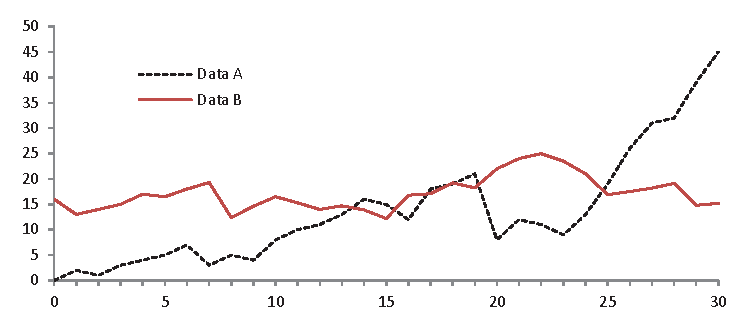
\includegraphics[width=\textwidth]{fig1.eps}
% \caption{A figure caption is always placed below the illustration.
% Please note that short captions are centered, while long ones are
% justified by the macro package automatically.} \label{fig1}
% \end{figure}

% \begin{theorem}
% This is a sample theorem. The run-in heading is set in bold, while
% the following text appears in italics. Definitions, lemmas,
% propositions, and corollaries are styled the same way.
% \end{theorem}
%
% the environments 'definition', 'lemma', 'proposition', 'corollary',
% 'remark', and 'example' are defined in the LLNCS documentclass as well.
%
% \begin{proof}
% Proofs, examples, and remarks have the initial word in italics,
% while the following text appears in normal font.
% \end{proof}
% For citations of references, we prefer the use of square brackets
% and consecutive numbers. Citations using labels or the author/year
% convention are also acceptable. The following bibliography provides
% a sample reference list with entries for journal
% articles~\cite{ref_article1}, an LNCS chapter~\cite{ref_lncs1}, a
% book~\cite{ref_book1}, proceedings without editors~\cite{ref_proc1},
% and a homepage~\cite{ref_url1}. Multiple citations are grouped
% \cite{ref_article1,ref_lncs1,ref_book1},
% \cite{ref_article1,ref_book1,ref_proc1,ref_url1}.
%
% ---- Bibliography ----
%
% BibTeX users should specify bibliography style 'splncs04'.
% References will then be sorted and formatted in the correct style.
%
% \bibliographystyle{splncs04}
% \bibliography{mybibliography}
%
\begin{thebibliography}{8}
% \bibitem{ref_article1}
% Author, F.: Article title. Journal \textbf{2}(5), 99--110 (2016)

% \bibitem{ref_lncs1}
% Author, F., Author, S.: Title of a proceedings paper. In: Editor,
% F., Editor, S. (eds.) CONFERENCE 2016, LNCS, vol. 9999, pp. 1--13.
% Springer, Heidelberg (2016). \doi{10.10007/1234567890}

% \bibitem{ref_book1}
% Author, F., Author, S., Author, T.: Book title. 2nd edn. Publisher,
% Location (1999)

% \bibitem{ref_proc1}
% Author, A.-B.: Contribution title. In: 9th International Proceedings
% on Proceedings, pp. 1--2. Publisher, Location (2010)

% \bibitem{ref_url1}
% LNCS Homepage, \url{http://www.springer.com/lncs}. Last accessed 4
% Oct 2017
\end{thebibliography}
\end{document}
